\documentclass[12]{article}
\usepackage{chngcntr}

\usepackage{gensymb}
\usepackage{float}
\usepackage{float}
\usepackage{booktabs}
\usepackage{multirow}
\usepackage{amsmath}
\usepackage[utf8]{inputenc}
\usepackage[T1]{fontenc}
\usepackage{hyperref}
\hypersetup{
    colorlinks,
    citecolor=black,
    filecolor=black,
    linkcolor=blue,
    urlcolor=blue
}

\setlength{\oddsidemargin}{0.25 in}
\setlength{\evensidemargin}{-0.25 in}
\setlength{\topmargin}{-0.6 in}
\setlength{\textwidth}{6.5 in}
\setlength{\textheight}{8.5 in}
\setlength{\headsep}{0.75 in}
\setlength{\parindent}{0 in}
\setlength{\parskip}{0.1 in}
\usepackage{geometry}
\usepackage{textcomp}
\usepackage[table,xcdraw]{xcolor}
\counterwithin{figure}{subsection}
\usepackage{graphicx}
\usepackage[inkscapeformat=pdf,inkscapelatex=false]{svg}
\graphicspath{ {./figs/} }

\begin{document}
\begin{titlepage}
\newcommand{\HRule}{\rule{\linewidth}{0.5mm}}
\setlength{\topmargin}{0 in}
\begin{center}
\begin{figure}[!h]
\centering

\includegraphics [width=0.3\textwidth]{eelogo.png}
\end{figure}

\vspace{10mm}
\Huge{MIDDLE EAST TECHNICAL UNIVERSITY}\\
\vspace{5mm}
{\LARGE ELECTRICAL \& ELECTRONICS ENGINEERING}\\

\HRule\\[0.4cm]
\textsc{\Large{EE463 - STATIC POWER CONVERSION I}}\\
\textsc{\Large{Hardware Project - AC to DC Motor Drive\\}}
\textsc{\Large{Simulation Report\\}}
\HRule\\[0.4cm]

\vspace{3mm}

\end{center}
\begin{minipage}{1\textwidth}
		\begin{flushleft}
			\large
			Emre Deniz  \textsc{Şenel - 2167237}\\
			Fahri \textsc{Türedi - 2167435}\\
			Ogün \textsc{Altun - 2165785}
			
		\end{flushleft}
	\end{minipage}

\vspace{10mm}
\begin{center}
\large{04.12.2019}
\end{center}
\end{titlepage}

\tableofcontents
\newpage

\section{Introduction}
naber
\counterwithin{figure}{section}
\section{Problem Definition}
In the project, it is required to drive a DC motor with AC voltage from variac. Motor will be connected to a DC generator that will be connected to a kettle which will boil water so that we can drink tea.

DC motor can be observed in the Figure \ref{motor-set} below:

\begin{center}
\begin{figure}[H]
\centering
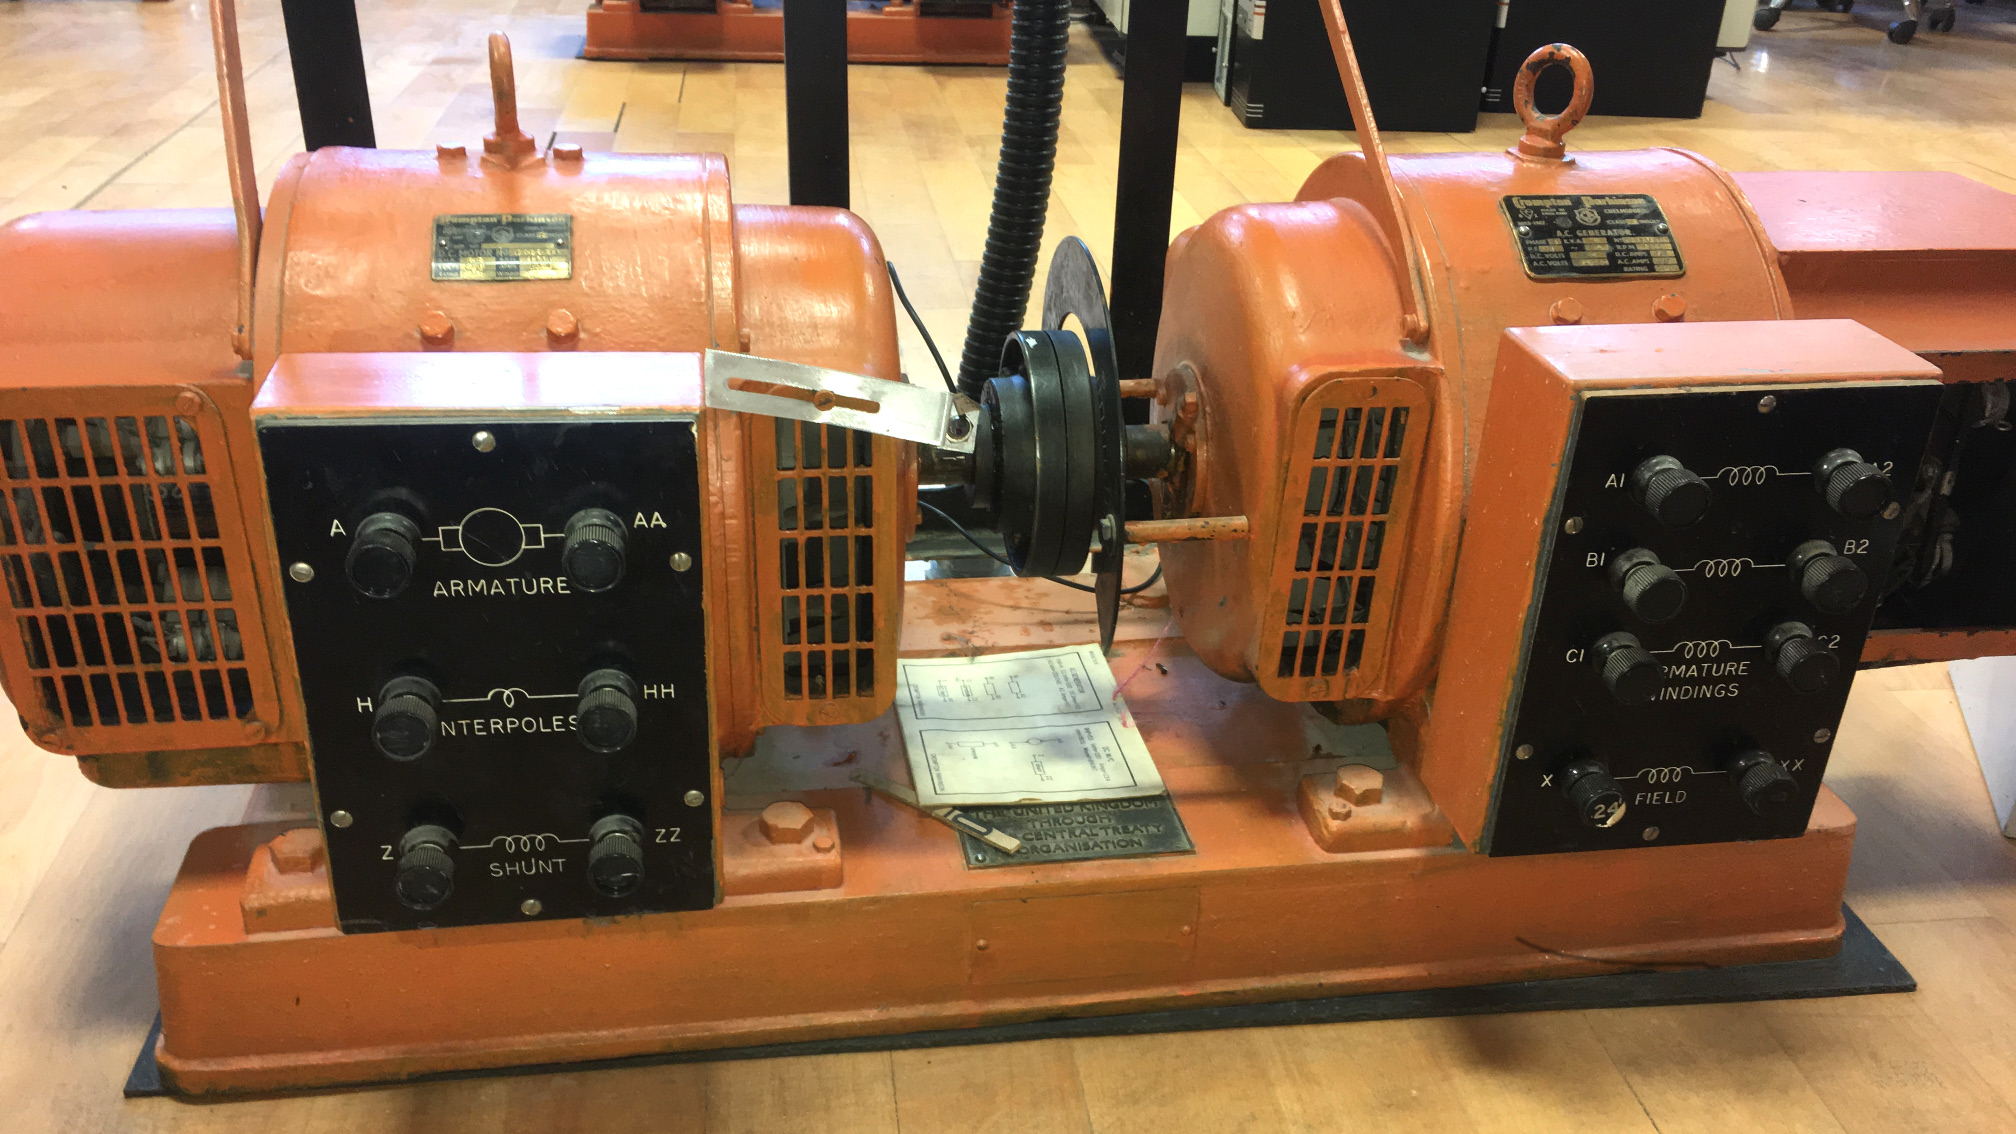
\includegraphics [width= 12 cm ]{motor-set}
\caption{DC Motor}
\label{motor-set}
\end{figure}
\end{center}

Parameters of the DC Motor:
\begin{itemize}
    \item Armature Winding: 0.8 \ohm, 12.5 mH
    \item Shunt Winding: 210 \ohm, 23 H
    \item Interpoles Winding: 0.27 \ohm, 12 mH
\end{itemize}

Requirements are:
\begin{itemize}
    \item Input is single-phase or three-phase AC Voltage
    \item Output, $V_{dc,max} < 180 V$
\end{itemize}

\counterwithin{figure}{subsection}
\section{A Brief Introduction of Possible Topologies}
In the project, topology is chosen among three possible solutions. They are: Single phase fully-controlled rectifier, three-phase fully-controlled rectifier and three-phase diode rectifier with buck converter. In this part, a brief introduction of each topology is provided. Expected theoretical voltage output is calculated.
\subsection{Single Phase Thyristor}
Thyristor rectifier topologies are generally suitable for high power demanding applications like HVDC transmission systems. The topology consists of 4 thyristors. Its operation is similar to Single Phase Diode Rectifier. However, in contrast to the constant, or in other words uncontrollable, average output voltage characteristic of diode rectifiers, the Single Phase Thyristor Rectifier topology allows controlled operation. The average output voltage of the rectifier can be controlled by adjusting the firing angle of the thyristors. Hence, we can achieve AC to variable DC conversion with this topology. The firing of the thyristors is controlled by applying a pulse signal the gate terminals of the devices. In order to synchronize the firing times of the thyristors, the zero crossings of the input ac waveform should be detected. There should be 180\degree phase shift between the firing times of the two set of thyristors.
\subsubsection{Operation and Structure}
The Single Phase Fully-Controlled Rectifier topology is given in Figure \ref{SingleThyristor}.
\begin{center}
\begin{figure}[H]
\centering
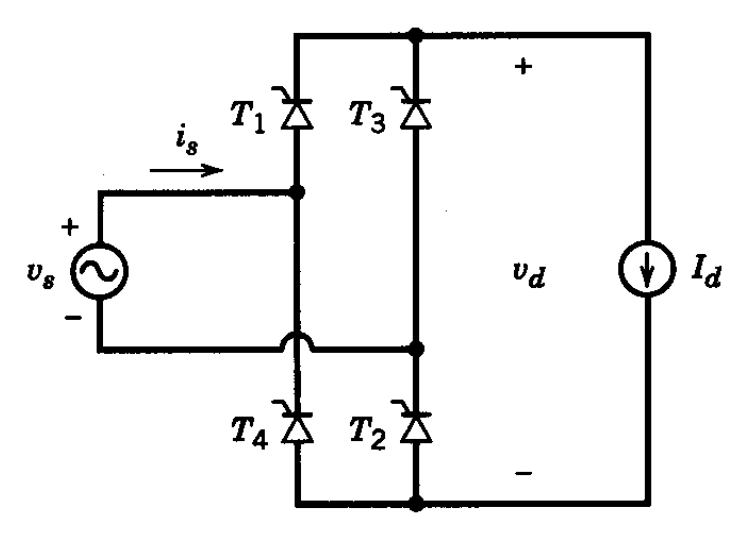
\includegraphics [width= 12 cm ]{singlephthyristor.png}
\caption{Single Phase Fully-Controlled Rectifier Structure}
\label{SingleThyristor}
\end{figure}
\end{center}

During the positive half cycle of the input voltage thyristors T1 and T2 conducts the current after they are fired. In the negative half cycle of the input voltage, the current commutates from thyristors T1 and T2 to thyristors T3 and T4. The zero crossings of the input voltage waveform should be detected to synchronize the firing times of thyristors. By controlling the firing angle of the thyristors, the average of the output voltage can be controlled.

There are basically two operation modes of this rectifier topology: rectification mode and inverter mode.
In rectification mode, the average output voltage and current of the rectifier topology is positive. In this mode, power flows from ac (input/grid) side to the dc (output/load) side of the rectifier.

In inverter mode of operation, the average output voltage becomes negative while the output current is still positive. Hence, the power flows from dc (output/load) side to ac (input/grid) side. In other words, the rectifier supplies back power to the grid. In order for this rectifier topology to operate in this mode, there should exist an active source element at the output/load side of the topology. 

Theoretical calculation for the average output voltage of the topology is given below:
\begin{equation}
    V_{avg} = \frac{2 \sqrt{2}}{\pi} V_{ph} \cos{\alpha} 
\end{equation}
A capacitor with large capacitance value can be connected in the load side of the rectifier in order to filter the output voltage, and reduce the output voltage ripple.

\subsubsection{Advantages}
\begin{itemize}
    \item The output voltage can be fully controlled by controlling the firing angles the thyristors.
    \item The structure of the topology is quite simple. It consists of only 4 thyristors.
    \item Its operation is also quite simple compared to three phase topologies and buck converter topology.
    \item It can be operated in four quadrant by connecting two Single Phase Thyristor Rectifier topologies back to back. When it is operated in its inverter mode, the rectifier can supply power back to the grid if an active source is available in the load side of the rectifier. In other words, the output voltage can become negative while the current is still positive.
    \item Driving the gates of the thyristors in this topology is relatively simple compared to three phase topologies.
    \item Relatively less number of components are required to construct the topology compared to three phase topologies. Only 4 thyristors and two gate drivers are required. Therefore, the topology is small in size.
\end{itemize}
\subsubsection{Disadvantages}
\begin{itemize}
    \item The output voltage ripple is quite high. The output voltage waveform follows the input voltage waveform. Hence, its ripple is equal to the input voltage ripple depending on the firing angle. In order to reduce the output voltage ripple, a large capacitor should be connected to the output of the rectifier.
    \item The harmonics in the input current are problematic in this topology. All odd harmonics exist in the input current waveform. This results in high THD value for the input current. In order to reduce the effects of those odd harmonics, a large source inductance should be added to the grid (input) side. However, the addition of the source side inductance effects the commutation time of the rectifier circuit. The commutation time increases with increasing source side inductance.
    \item In general, driving the gates of the thyristors is quite tedius and troublesome. A driver circuit is required to drive the gates of the thyristors. Also, gates should be fired at precisely correct angles in order to ensure the synchronous operation of the thyristors.
    \item The zero crossings of the input voltage waveform should be detected to synchronize the firing angles of the thyristors. 
\end{itemize}

\subsection{Three Phase Thyristor}
Second topology constructed with thyristors is three phase fully controlled rectifier. It is named as it is because with thyristors the output voltage can be controlled without having any dc-dc converter at the output. In the lectures, three phase thyristors are covered, operation philosophy, advantages and disadvantages with explanations can be followed below:
\subsubsection{Operation and Structure}
In the Figure \ref{fig:ThreeThyristor} below, the topology can be observed:

\begin{center}
\begin{figure}[H]
\centering
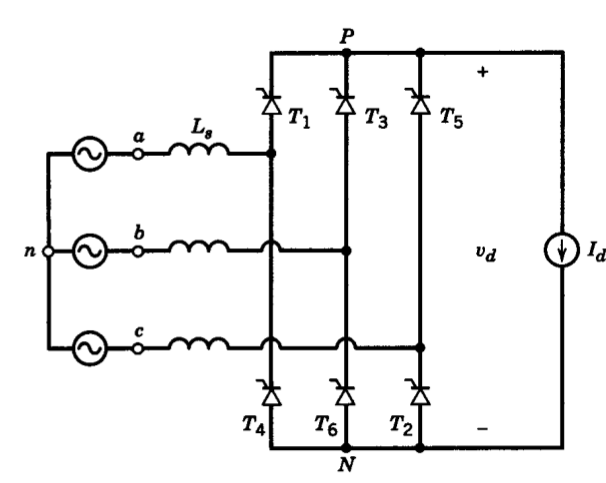
\includegraphics [width= 12 cm ]{ThreeThyristor.png}
\caption{Three Phase Fully-Controlled Rectifier Structure}
\label{fig:ThreeThyristor}
\end{figure}
\end{center}

In the three phase fully-controlled rectifier, six thyristors are used. Using gate signal generators, thyristors are fired in order to control output voltage. Theoretical calculation of output voltage is below:

\begin{equation}
    V_{avg} = \frac{3 \sqrt{2}}{\pi} V_{LL} \cos{\alpha} 
\end{equation}

\subsubsection{Advantages}
\begin{itemize}
    \item In this topology, output voltage can be controlled without any additional converter.
    \item Output ripple of this topology is respectively low. In order to decrease the ripple, a lower capacitor can be used in this topology.
    \item Third harmonic of input current is not observed in this topology. So, THD is respectively low.
    \item This topology can be used in inverter mode. Therefore, to obtain four quadrant operation, back to back three phase fully-controlled rectifiers can be utilized.
\end{itemize}

\subsubsection{Disadvantages}
\begin{itemize}
    \item This topology is built of six thyristors. Thyristors are expensive components comparing to the normal diodes. Therefore, this topology is more expensive than other options.
    \item In order to drive this rectifier, six different gate signals have to be used. This requires gate drivers and more components. It increases the cost, and it complicates the structure.
    \item Synchronization of gate drivers is hard. A zero crossing detector should be used in order to control it, it increases the cost and it makes the topology difficult.
\end{itemize}

\subsection{Three Phase Diode Rectifier with Buck Converter}
\subsubsection{Operation and Structure}
This topology consists of two parts. First part rectifies three phase ac grid voltage to low-ripple dc voltage. In the second part, we apply a buck converter and control our output voltage with duty cycle of switch. The first part of this topology is three phase diode rectifier. In the Figure \ref{fig:ThreeDiode} below the topology of three phase diode rectifier can be observed.

\begin{center}
\begin{figure}[H]
\centering
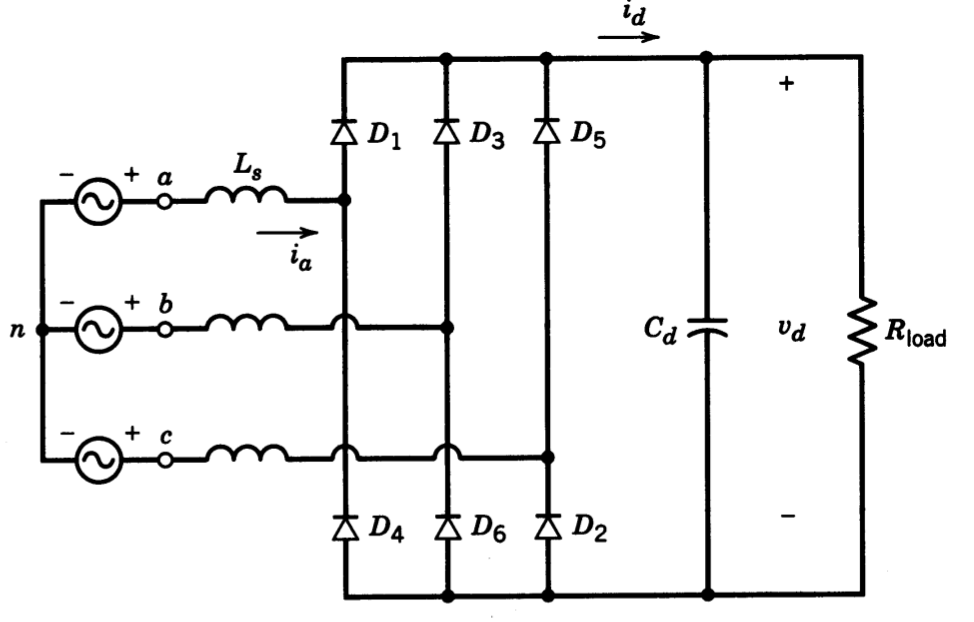
\includegraphics [width= 12 cm ]{threediode.png}
\caption{Three Phase Diode Rectifier Structure}
\label{fig:ThreeDiode}
\end{figure}
\end{center}

In three phase diode rectifier, one of upper diodes and one of bottom diodes conducts according to the phase voltage levels. In this topology we have no control of average output voltage. Below, theoretical output voltage can be observed.

\begin{equation}
    V_{avg} = \frac{3 \sqrt{2}}{\pi} V_{LL}
\end{equation}

In the Figure \ref{Buck} below, topology of step down converter can be examined.

\begin{center}
\begin{figure}[H]
\centering
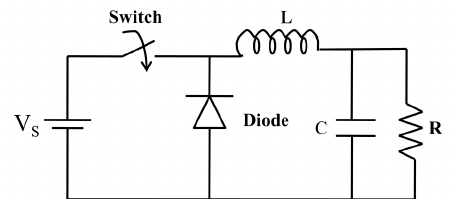
\includegraphics [width= 12 cm ]{buck.png}
\caption{Buck Converter Structure}
\label{Buck}
\end{figure}
\end{center}


Second part of this structure is buck converter. Buck converter basically step downs the input dc voltage to a desired level. In order to control output voltage, a MOSFET driven by a gate signal generator is used. Below, theoretical output voltage can be observed, D stands for duty cycle.

\begin{equation}
    V_{out} = DV_{in}
\end{equation}

Connecting diode rectifier and buck converter results in average voltage:
\begin{equation}
   V_{avg} = \frac{3 \sqrt{2}}{\pi} V_{LL} D
\end{equation}



\subsubsection{Advantages}
\begin{itemize}
    \item In this topology output voltage ripple is respectively low. 
    \item This topology requires only one gate signal which will be provided to drive buck converter. Thus, this is system is less complicated comparing to other topologies. Also, in this topology there is no need of synchronizing the signals.
    \item This topology consists of six diodes and a buck converter, this system is less expensive comparing to thyristor rectifiers.
    \item Since our motor is an LR load, we do not need to construct LC filter at the output of buck converter. This means this topology can be built easier.
\end{itemize}

\subsubsection{Disadvantages}
\begin{itemize}
    \item This topology does not support four quadrant operation. Diode rectifier can work in only one quadrant, so there is no way to obtain four quadrant.
    \item Theoretically, the expected efficiency is lower than thyristor cases because we use external diode in the buck converter.
\end{itemize}
\section{Topology Selection and Reasoning}
merhaba
\section{Simulations}
In this part, simulations of the selected topology will be provided. Simulations will be provided in three parts, in the first part we provide three-phase diode rectifier simulations and results. In the second part buck converter results and simulations are provided. In the last part, the circuit as a whole will be examined.

\subsection{Simulations of Three Phase Diode Rectifier}

In the Figure \ref{Schematic3diode} below, schematic of Simulink simulation can be observed. This simulation is constructed with a single resistance at the output. This simulation does not contain line impedances, and diodes are ideal.

\begin{center}
\begin{figure}[H]
\centering
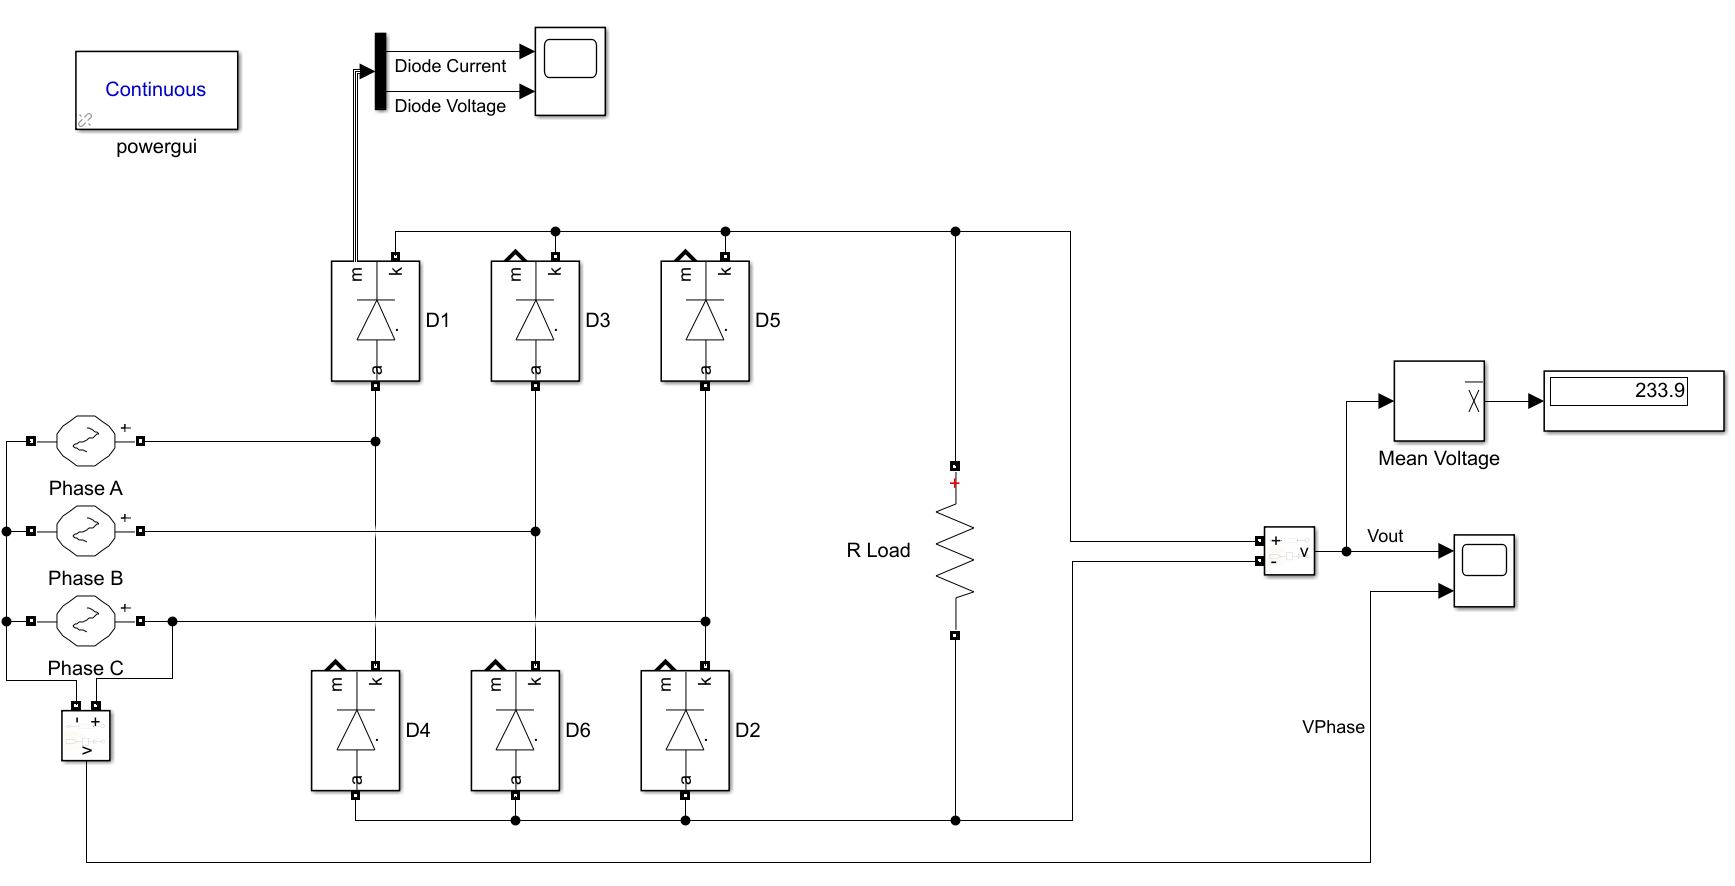
\includegraphics [width= 15 cm ]{diodetopology}
\caption{Schematic of Three Phase Diode Rectifier}
\label{Schematic3diode}
\end{figure}
\end{center}

It is given that the output voltage of the whole converter $V_{max}$ must be less than $180V_{dc}$. We limited the duty cycle of buck converter to 80\%. Then, $V_{rectifier,av}$ can be calculated as below formula.

\[V_{in,buck} = V_{rec,ac} = \frac{V_{out}}{D}=225V\]

$V_{RMS}$ can be calculated as:

\[V_s = 225\frac{\pi}{3\sqrt{6}}=96.2 V_{rms}\]

So, the input voltage was chosen as $100V_{rms}$

In the Figure \ref{Voltage3diode} below, input phase voltage and output voltage can be observed.
\begin{center}
\begin{figure}[H]
\centering
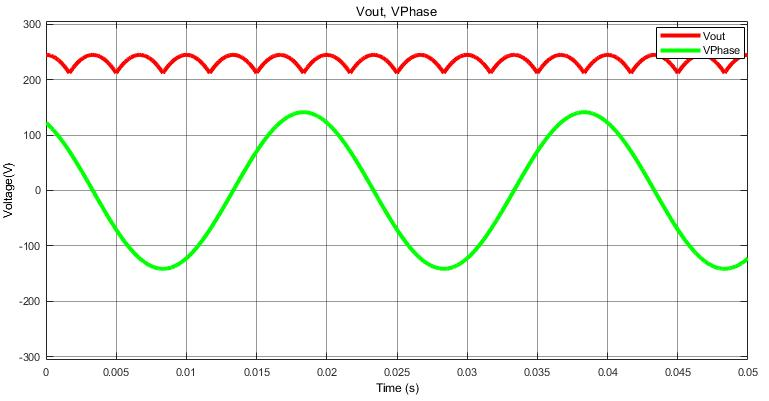
\includegraphics [width= 12 cm ]{voltageout}
\caption{Voltage Output and Voltage Input of Three Phase Diode Rectifier}
\label{Voltage3diode}
\end{figure}
\end{center}

Input voltage of a three-phase diode rectifier has frequency of 50, Turkish Grid Frequency. However, as we observe in the output, output has six times of input frequency. Thus, this topology can be named as six pulse diode rectifier. Output voltage ripple is respectively low in this case. It can be simulated as 32.8 V. Moreover, this topology does not have triplen harmonics in input current. This results in lower THD, and better power quality. THD of this topology is simulated as 31.8\%

Input and output current waveforms can be observed from Figure \ref{Current3diode} below.

\begin{center}
\begin{figure}[H]
\centering
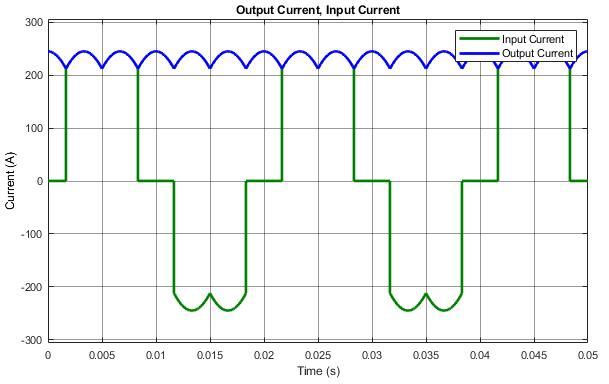
\includegraphics [width= 12 cm ]{inputcurrent}
\caption{Input Current and Output Current of Three Phase Diode Rectifier}
\label{Current3diode}
\end{figure}
\end{center}

Component selection will be based on stresses and limits. In the Figure \ref{Diode3diode} below, diode stresses can be observed.

\begin{center}
\begin{figure}[H]
\centering
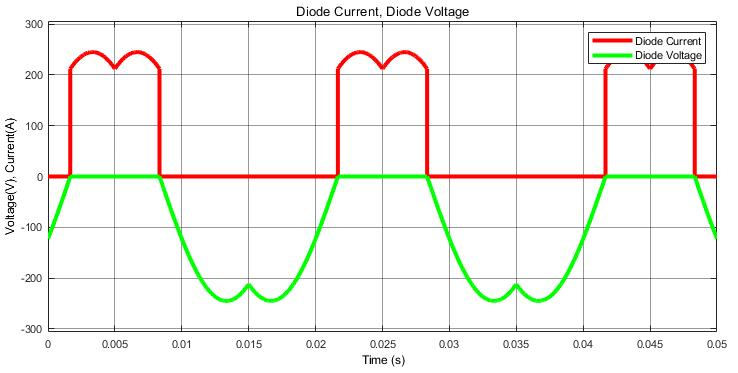
\includegraphics [width= 12 cm ]{currentdiode}
\caption{Diode Current and Diode Voltage of a Diode}
\label{Diode3diode}
\end{figure}
\end{center}

It is obvious that our diodes have to be able to carry peak current of 250A. However, this stress is for the ideal case with output resistance of 1\ohm. This value will be less when we add the buck converter, and the DC Machine. Also, our diodes should have reverse voltage of minimum -250V.

\subsection{Simulations of Buck Converter}
The Simulink simulation schematic of the Buck Converter circuit topology is given in Figure \ref{voltcurrentbuckout}. The topology is simulated to observe the output voltage and current waveforms, diode current and voltage waveforms and MOSFET voltage and current waveforms.

In the simulations, the switching frequency of the MOSFET is chosen 1 kHz with 10\% duty cycle. Since initially dc motor is at standstill, there is no back emf produced by the motor, which will limit the output current of the Buck Converter. Therefore, we should be careful about the start-up current of the dc motor. In order to limit the output current at start-up, we have decided to initially set the duty cycle of the control signal to be 0.1 . Thus, it is ensured that the output current does not exceed the rated current of the dc motor, which is provided 23.4 A. We plan to steadily increase the duty cycle of the control signal from 0.1 (10\%) to 0.8 (80\%) in a finite duration until the back emf of the motor builts up while it is reaching its rated speed, and hence reach steady state condition. Thereafter, we can control the output dc voltage of the converter circuit to obtain variable DC output converter. The input voltage is applied from a dc voltage source with 225 V as computed in the subsection 4.1. Since the dc motor itself is a big RL load, it is thought to be unnecessary to add an LC filter at the output for the Buck Converter. Hence, we have modelled the buck converter without LC filter at the output. The output of the Buck Converter circuit is loaded with the resistance (R) and inductance (L) ratings of the DC Motor to be driven. A dc voltage source representing the back emf voltage of the dc motor is also added at the output. However, it is set to 0.1 V in order to obtain the start-up current and voltage waveforms of the output load, MOSFET and freewheeling diode. The observed peak and average values of the current and voltage waveforms across the MOSFET and diode in simulations will be used in the component selection part to select the components with the suitable ratings to our circuit.

\begin{center}
\begin{figure}[H]
\centering
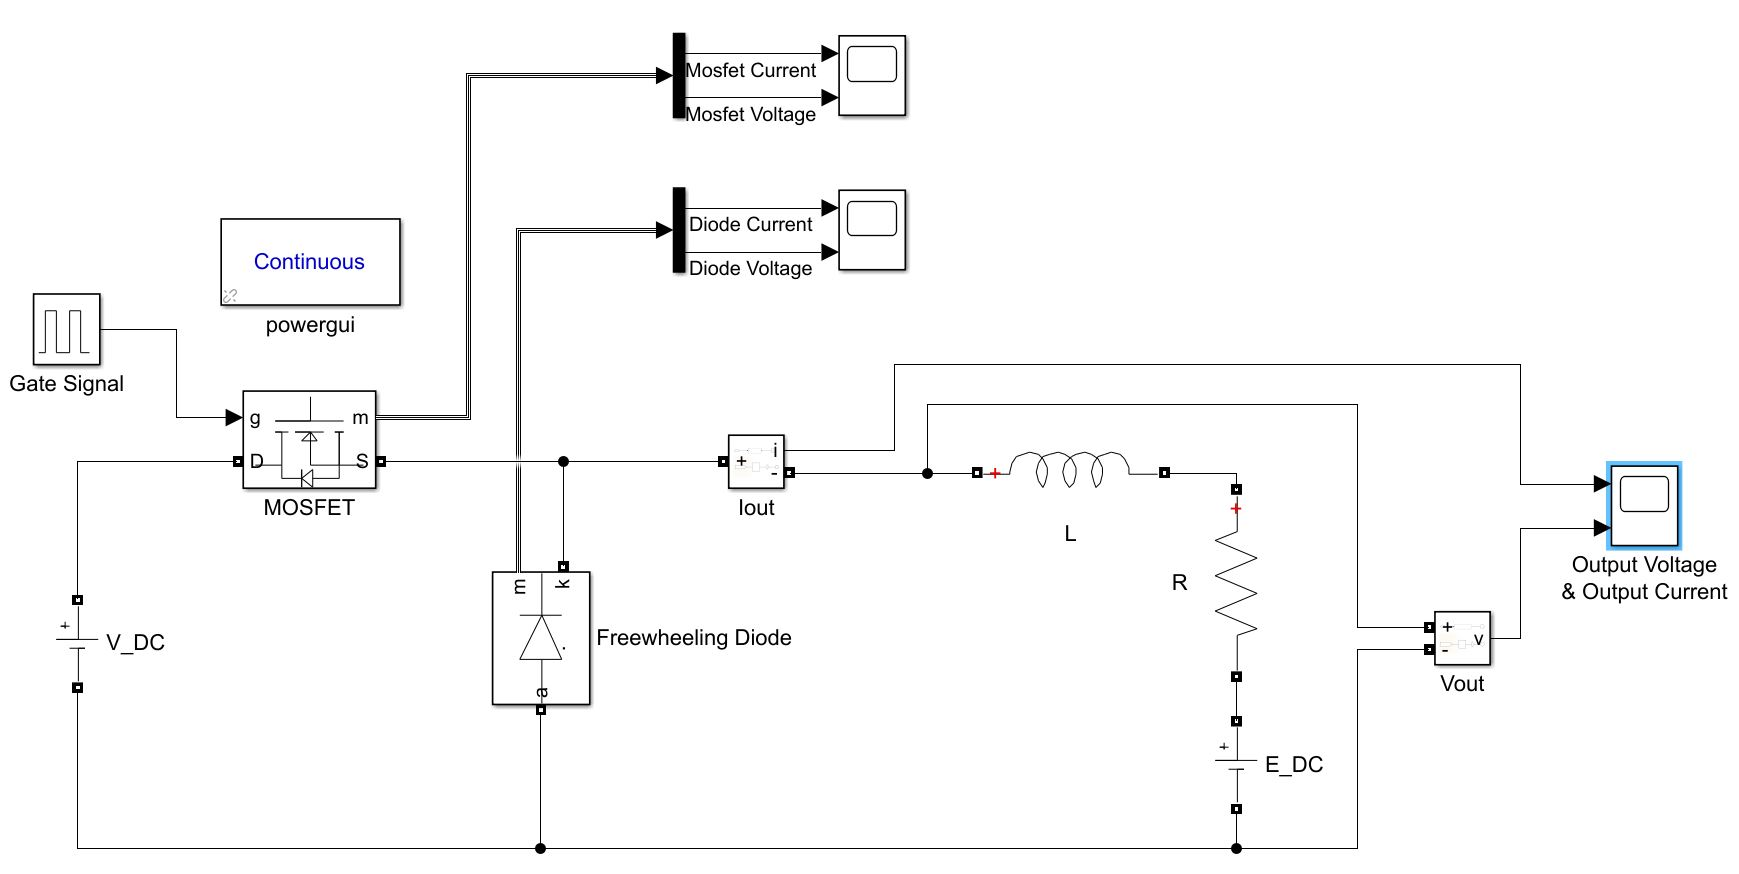
\includegraphics [width= 12 cm ]{voltcurrentbuckout}
\caption{Schematic of Buck Converter}
\label{voltcurrentbuckout}
\end{figure}
\end{center}

In the Figure \ref{buckvoltagecurrentout}, the output voltage and current waveforms of the Buck Converter circuit, obtained from simulations, are given.

At the output of the Buck Converter, a square wave voltage waveform is observed. The ripple in the output voltage is measured to be close to 225 V. However, the ripple in the output current of the circuit is quite small.
\begin{center}
\begin{figure}[H]
\centering
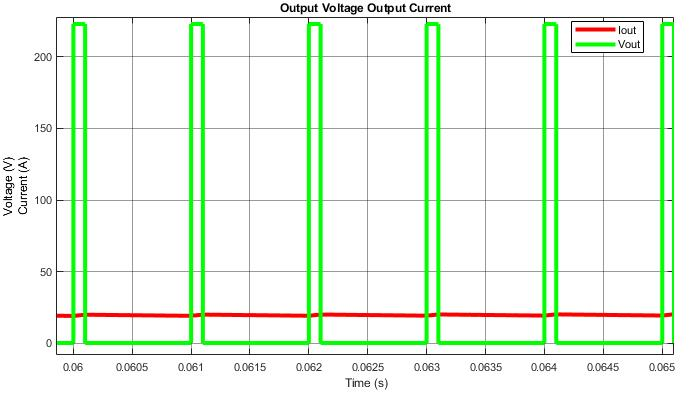
\includegraphics [width= 12 cm ]{buckvoltagecurrentout}
\caption{Buck Converter Output Voltage and Output Current Waveforms}
\label{buckvoltagecurrentout}
\end{figure}
\end{center}

MOSFET voltage and current waveforms are given in Figure \ref{mosfetcurrvolt} below.

\begin{center}
\begin{figure}[H]
\centering
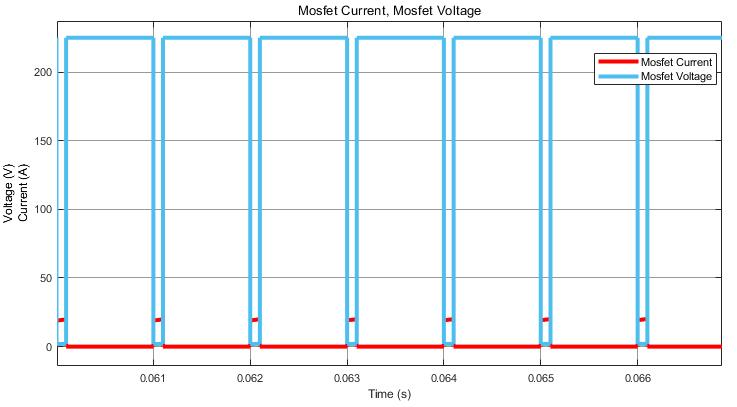
\includegraphics [width= 12 cm ]{mosfetcurrvolt}
\caption{MOSFET Voltage and Current Waveforms}
\label{mosfetcurrvolt}
\end{figure}
\end{center}

The Figure \ref{freediodecurrvolt} shows the voltage and current waveforms across the freewheeling diode.
\begin{center}
\begin{figure}[H]
\centering
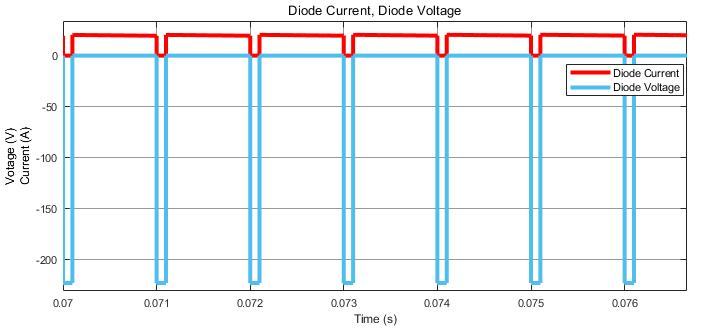
\includegraphics [width= 12 cm ]{freediodecurrvolt}
\caption{Freewheeling Diode Voltage and Current Waveforms}
\label{freediodecurrvolt}
\end{figure}
\end{center}

\subsection{Simulations of Rectifier \& Buck Converter}

In the Figure \ref{diodebuck} below, we can observe the whole circuit consists of diode rectifier and buck converter. In the schematic, we used an RL load with dc voltage, it is basically a motor model. Displays show average values of diode voltage and inputs. This values are critical for component selection.

\begin{center}
\begin{figure}[H]
\centering
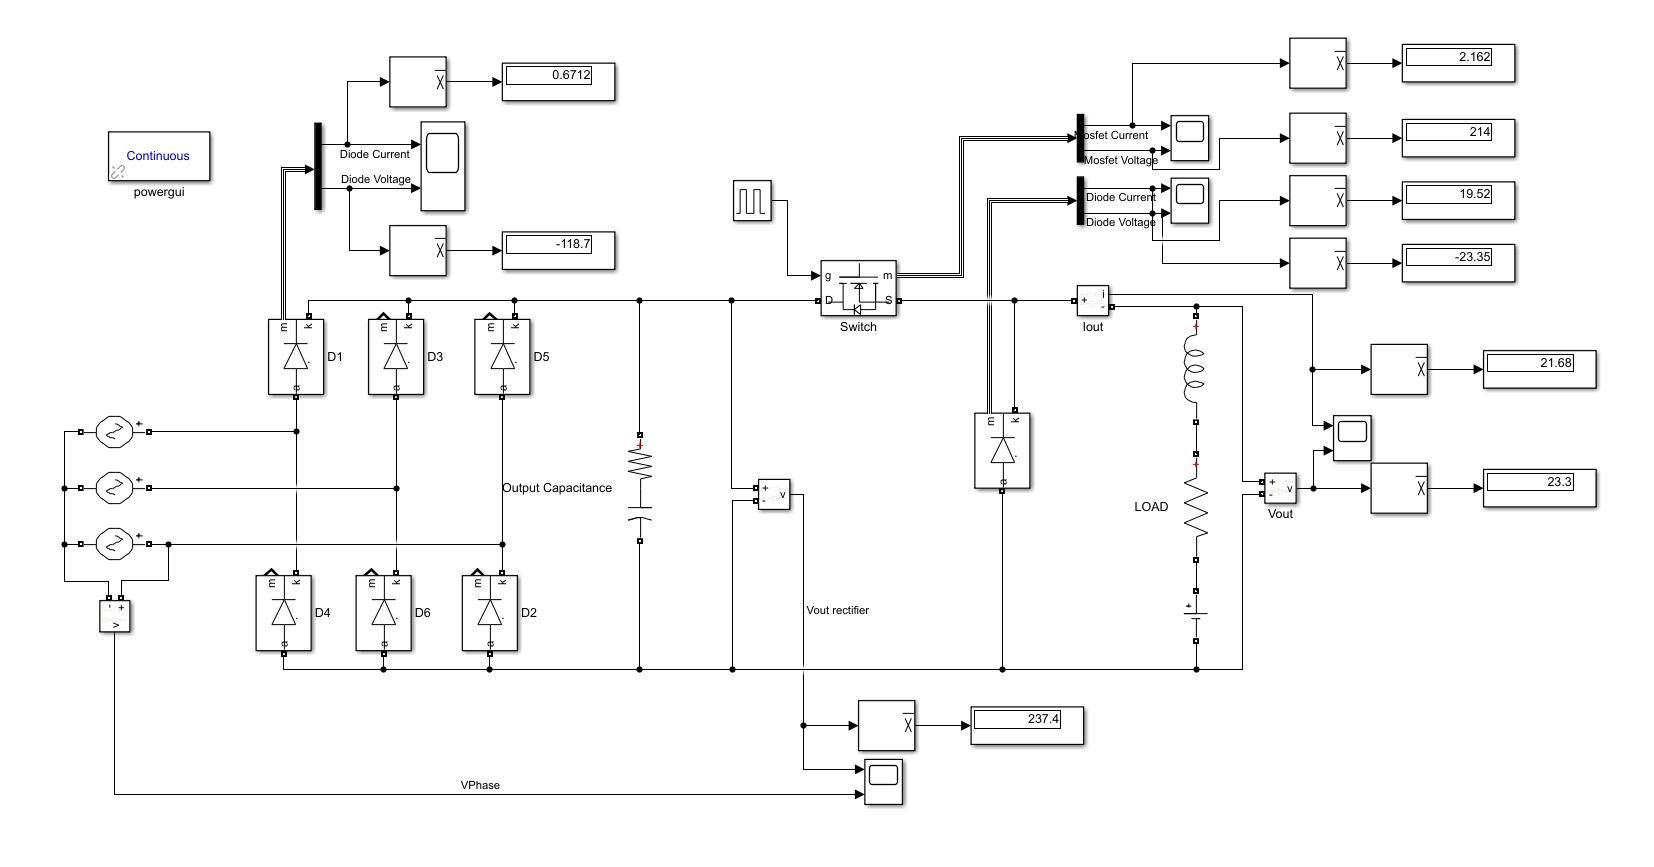
\includegraphics [width= 12 cm ]{diodebuck}
\caption{Schematic of Whole Circuit}
\label{diodebuck}
\end{figure}
\end{center}

In the Figure below \ref{wholeoutput}, output voltage and current for start up can be observed. It is taken at duty cycle of 0.1

\begin{center}
\begin{figure}[H]
\centering
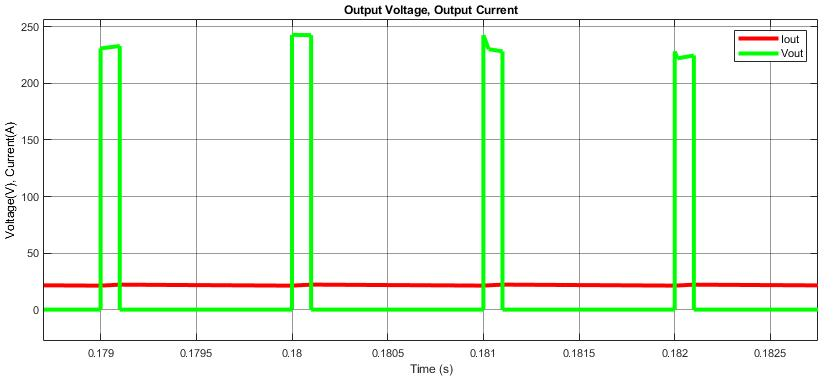
\includegraphics [width= 12 cm ]{wholeoutput}
\caption{Output Voltage and Current Waveforms of Converter}
\label{wholeoutput}
\end{figure}
\end{center}

In the Figure \ref{inputdiodewave} below, we can see transient waveform of the input diode. At start-up, maximum current is around 24 Amperes, and reverse voltage is around -250 Volts.

\begin{center}
\begin{figure}[H]
\centering
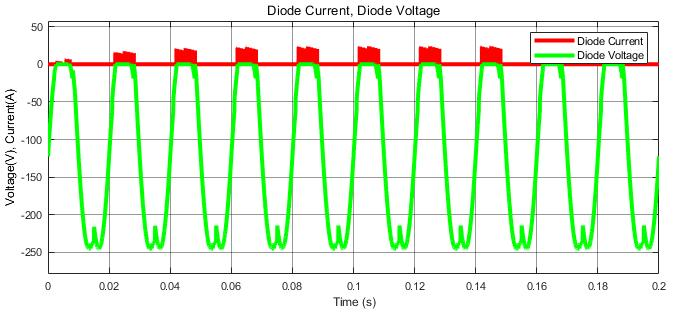
\includegraphics [width= 12 cm ]{inputdiodewave}
\caption{Rectifier Diode Voltage and Current Waveforms}
\label{inputdiodewave}
\end{figure}
\end{center}

In the Figure \ref{wholemosfet} below, we can observe MOSFET stresses, average current is around 3 Amperes and blocking voltage is around 214 Volts at start-up.
\begin{center}
\begin{figure}[H]
\centering
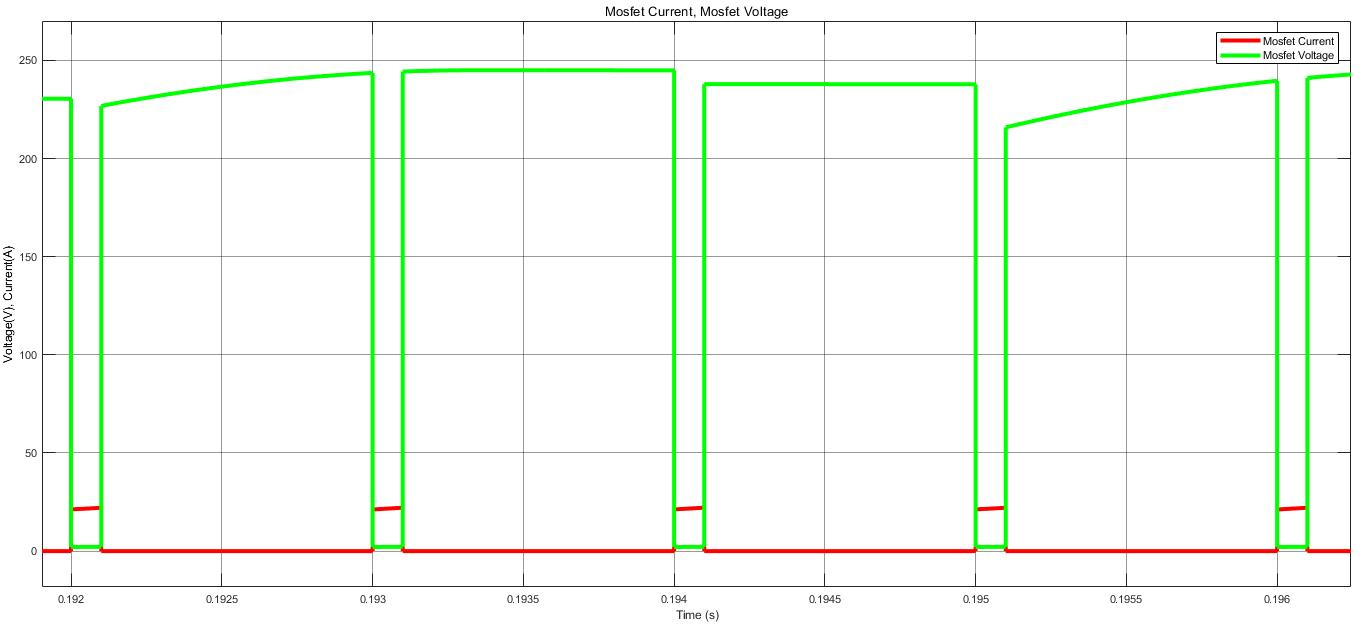
\includegraphics [width= 12 cm ]{wholemosfet}
\caption{MOSFET Voltage and Current Waveforms at Start-Up, D=10\%}
\label{wholemosfet}
\end{figure}
\end{center}

In the Figure \ref{diodesteady} below, we can observe the freewheeling diode stresses, average current is around 25 Amperes and blocking voltage is around 220 Volts at start-up.
\begin{center}
\begin{figure}[H]
\centering
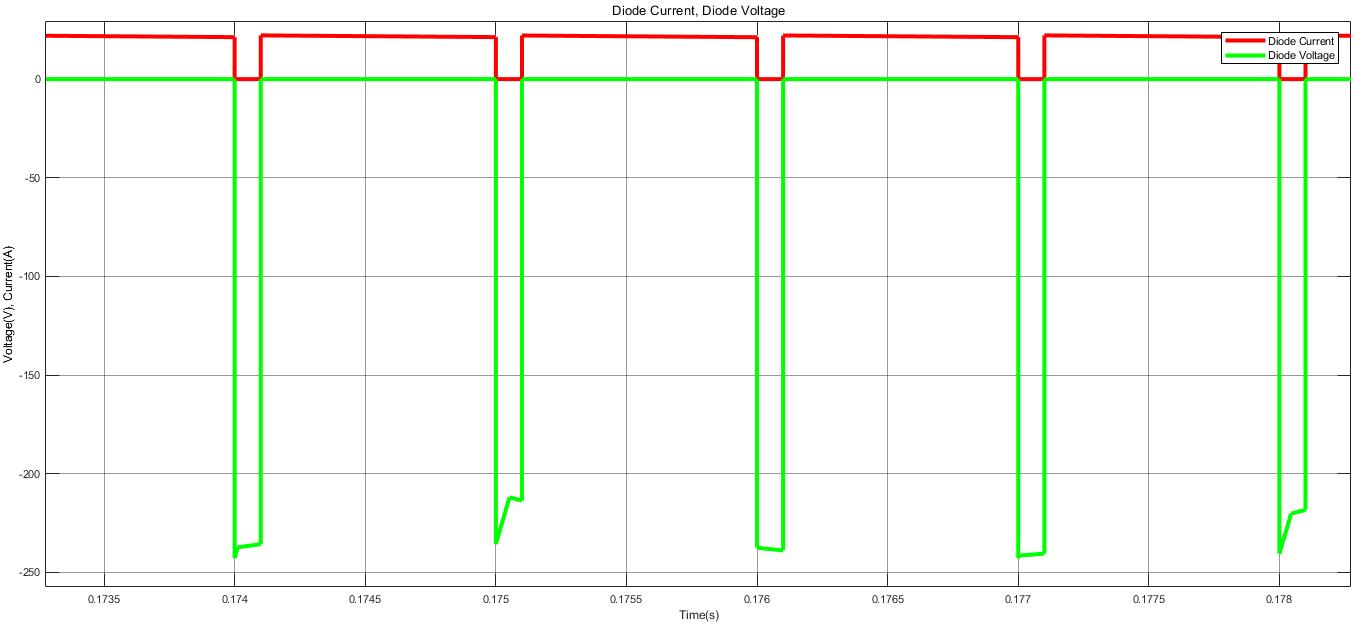
\includegraphics [width= 12 cm ]{diodesteady}
\caption{Freewheeling Diode Voltage and Current Waveforms at Start-Up, D=10\%}
\label{diodesteady}
\end{figure}
\end{center}

In the Figure \ref{diodefinal} below, we can observe the freewheeling diode stresses, average current is around 20 Amperes and the reverse voltage is around 25 Volts at steady-state.
\begin{center}
\begin{figure}[H]
\centering
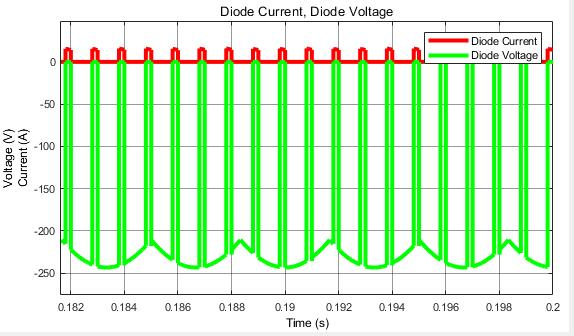
\includegraphics [width= 12 cm ]{finalfwd}
\caption{Freewheeling Diode Voltage and Current Waveforms at Steady State, D=80\%}
\label{diodefinal}
\end{figure}
\end{center}

In the Figure \ref{mosfetfinal} below, we can observe the MOSFET stresses, average current is around 12 Amperes and the reverse voltage is around 50 Volts at steady-state.
\begin{center}
\begin{figure}[H]
\centering
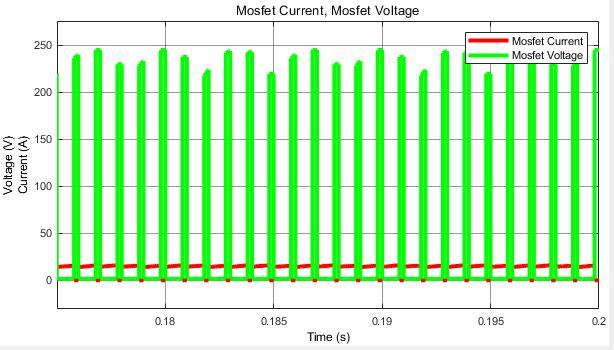
\includegraphics [width= 12 cm ]{finalmosfet}
\caption{MOSFET Voltage and Current Waveforms at Steady State, D=80\%}
\label{mosfetfinal}
\end{figure}
\end{center}

Simulations show that, critical points that need attention is:
\begin{itemize}
    \item At start-up, current of freewheeling diode and voltage of MOSFET is critical. We paid attention when we select the components.
    \item At steady-state, voltage of freewheeling diode and rectifier's diode current is critical. Also, MOSFET's current is critical. We paid attention to these parameters 
\end{itemize}






\section{Component Selection}

We have simulated the Simulink Model such that input voltage and currents are similar to rated values. After completing the simulations, we have selected the components that we are going to use in the project.

Since the “Buck Converter” MOSFET will conduct at around 80\% duty cycle after reaching rated speed, we decided to select a MOSFET that can carry up to 25-30 A average current. The voltage rating of the MOSFET must be bigger than 250V according to the simulation results. When we looked at the available components in the laboratory, we thought that \href{http://ixapps.ixys.com/Datasheet/DS100254B(IXGH24N60C4D1).pdf}{IXGH24N60C4D1} N Channel IGBT Transistor can be a good selection for us. 

To decide which diode that we will use, we have followed the same procedure. The free-wheeling diode in the buck converter will carry at 90\% duty cycle at start up. Therefore, it can carry 25 A current. The reverse voltage of this diode reaches up to 200 V average at rated speed and has 250V peak value. Providing required voltage and current rating, \href{http://ixapps.ixys.com/DataSheet/DSEI30-06A.pdf}{DSEI30-06A} has been selected for the free-wheeling diode of the buck converter.

The simulation results imply that diodes on the rectifier will carry average 10 A current which has 20-25 A peak value. Reverse voltage of rectifier diode has peak value of 245 V which is the peak of applied line to line voltage. By considering all these requirements, \href{http://ixapps.ixys.com/DataSheet/DSEI30-06A.pdf}{DSEI30-06A} is also a good selection for rectifier diodes. However, we think that \href{http://ixapps.ixys.com/DataSheet/DSEI12-06A.pdf}{DSEI12-06A} can also be used which has smaller but enough current rating. 

We decided to use a 100uF 400V capacitor at the output of the rectifier. \href{https://www.nichicon.co.jp/english/products/pdfs/e-ucs.pdf}{33 uF Capacitor}, we will use three in parallel.

\section{Conclusion}
In this project, our goal is to drive a DC motor with AC input. In the simulation report provided, we first investigated different topologies. Then, we selected our solution and simulated it in Simulink. Components that will be proper to our rectifier were chosen. This report shows that our solution is working in the theoretical and simulation level. Based on the simulations and the calculations, we will start to construct our project.
\end{document}